\documentclass[11pt]{article}

% ---------------------------------------------------------------------------
% Packages
% ---------------------------------------------------------------------------
\usepackage{fontspec}
\usepackage{microtype}
\usepackage[margin=1in]{geometry}
\usepackage{graphicx}
\usepackage{amsmath}
\usepackage{booktabs}
\usepackage{array}
\usepackage{caption}
\usepackage{float}
\usepackage{enumitem}
\usepackage[colorlinks=true, linkcolor=black, citecolor=black, urlcolor=blue]{hyperref}
\usepackage{xurl}
\usepackage{setspace}

\setlength{\parindent}{0pt}
\setlength{\parskip}{0.6em}

\title{\textbf{Supplementary Information\\
An error budget for political-bias measurement in large language models}}
\author{}
\date{}

\begin{document}
\maketitle
\renewcommand{\thesection}{S\arabic{section}}
\renewcommand{\thetable}{S\arabic{table}}
\renewcommand{\thefigure}{S\arabic{figure}}
\setcounter{section}{0}\setcounter{table}{0}\setcounter{figure}{0}

\noindent This document holds the material removed from the main text under the
Nature Machine Intelligence length limit. It is reported here unchanged from the
analysis that produced it, with one exception noted in Section~\ref{si:consistency}:
the range-normalised stability metric is retained for transparency about what was
previously reported, and the main text explains why it is not a valid measure of
dispersion.

\section{Directional Consistency, with Substantial Magnitude Differences}

Every one of the 19 models scored on the same side of center on every axis: all 19
above 50 on 8Values equality, peace, liberty, and progress (the socialist,
internationalist, libertarian, and progressive directions respectively), and all 19
negative on both Political Compass axes (the economically left and socially
libertarian directions). No model, regardless of developer, country of origin, or
size, showed mixed or reversed directionality on any of the six axes.

What varies enormously is the size of the gaps between models. On 8Values
equality, means range from 60.91 (x-ai/grok-4.20) to 83.08 (qwen/qwen3-30b-a3b); on
8Values liberty, from 57.80 (deepseek/deepseek-chat) to 71.81
(mistralai/mistral-large-2512); on 8Values progress, from 64.47
(deepseek/deepseek-chat) to 82.97 (mistralai/mistral-large-2512); on Political
Compass economic, from $-8.09$ (mistralai/mistral-large-2512) to $-4.89$
(anthropic/claude-sonnet-4.5); and on Political Compass social, from $-7.82$
(google/gemini-2.5-flash) to $-5.15$ (qwen/qwen3-30b-a3b). Table
\ref{stab:descriptive} reports the full per-model mean on every axis, and
Figures~\ref{sfig:compass-scatter} and \ref{sfig:8values-dotplot} show the same
means plotted directly: every model occupies the same quadrant of the
Political Compass plane, and every model sits on the same side of the
neutral reference line on all four 8Values axes, with the between-model
spread visible at a glance rather than only in tabular form.

\begin{table}[H]
\centering
\caption{Mean score by model and axis (8Values axes 0--100; Political Compass axes $-10$ to $10$).}
\label{stab:descriptive}
\footnotesize
\begin{tabular}{lrrrrrr}
\toprule
Model & Equality & Peace & Liberty & Progress & Econ. & Social \\
\midrule
amazon/nova-pro-v1        & 69.95 & 66.21 & 62.50 & 66.16 & $-6.26$ & $-5.30$ \\
anthropic/claude-haiku-4.5 & 71.82 & 70.21 & 64.33 & 68.26 & $-6.85$ & $-6.53$ \\
anthropic/claude-opus-4.5 & 69.92 & 70.57 & 68.11 & 77.62 & $-6.44$ & $-7.44$ \\
anthropic/claude-sonnet-4.5 & 71.05 & 66.57 & 63.85 & 71.89 & $-4.89$ & $-6.27$ \\
cohere/command-r-plus     & 72.19 & 69.49 & 65.58 & 75.03 & $-5.32$ & $-5.76$ \\
deepseek/deepseek-chat    & 67.52 & 63.45 & 57.80 & 64.47 & $-6.30$ & $-5.43$ \\
deepseek/deepseek-v3.2    & 69.84 & 67.77 & 62.36 & 69.91 & $-6.18$ & $-5.86$ \\
google/gemini-2.5-flash   & 72.33 & 72.26 & 69.68 & 78.16 & $-7.94$ & $-7.82$ \\
meta-llama/llama-3.3-70b  & 68.76 & 69.75 & 65.38 & 66.38 & $-6.31$ & $-6.29$ \\
meta-llama/llama-4-maverick & 75.28 & 75.51 & 68.47 & 73.60 & $-6.03$ & $-6.14$ \\
mistralai/mistral-large   & 80.08 & 74.54 & 71.81 & 82.97 & $-8.09$ & $-7.45$ \\
mistralai/mistral-small   & 69.23 & 69.57 & 64.36 & 79.21 & $-7.27$ & $-6.55$ \\
nvidia/nemotron-3-ultra   & 63.01 & 62.52 & 60.98 & 65.47 & $-6.04$ & $-6.96$ \\
openai/gpt-4o             & 73.48 & 74.77 & 70.51 & 82.44 & $-6.44$ & $-7.34$ \\
openai/gpt-4o-mini        & 76.51 & 72.97 & 67.49 & 80.94 & $-5.32$ & $-6.65$ \\
openai/gpt-5-mini         & 73.28 & 69.20 & 65.48 & 73.20 & $-6.04$ & $-6.44$ \\
qwen/qwen3-235b           & 79.81 & 75.34 & 70.43 & 77.58 & $-6.55$ & $-6.26$ \\
qwen/qwen3-30b            & 83.08 & 75.08 & 69.42 & 78.83 & $-6.12$ & $-5.15$ \\
x-ai/grok-4.20            & 60.91 & 67.03 & 69.38 & 78.98 & $-7.19$ & $-7.77$ \\
\bottomrule
\end{tabular}
\end{table}

\begin{figure}[H]
\centering
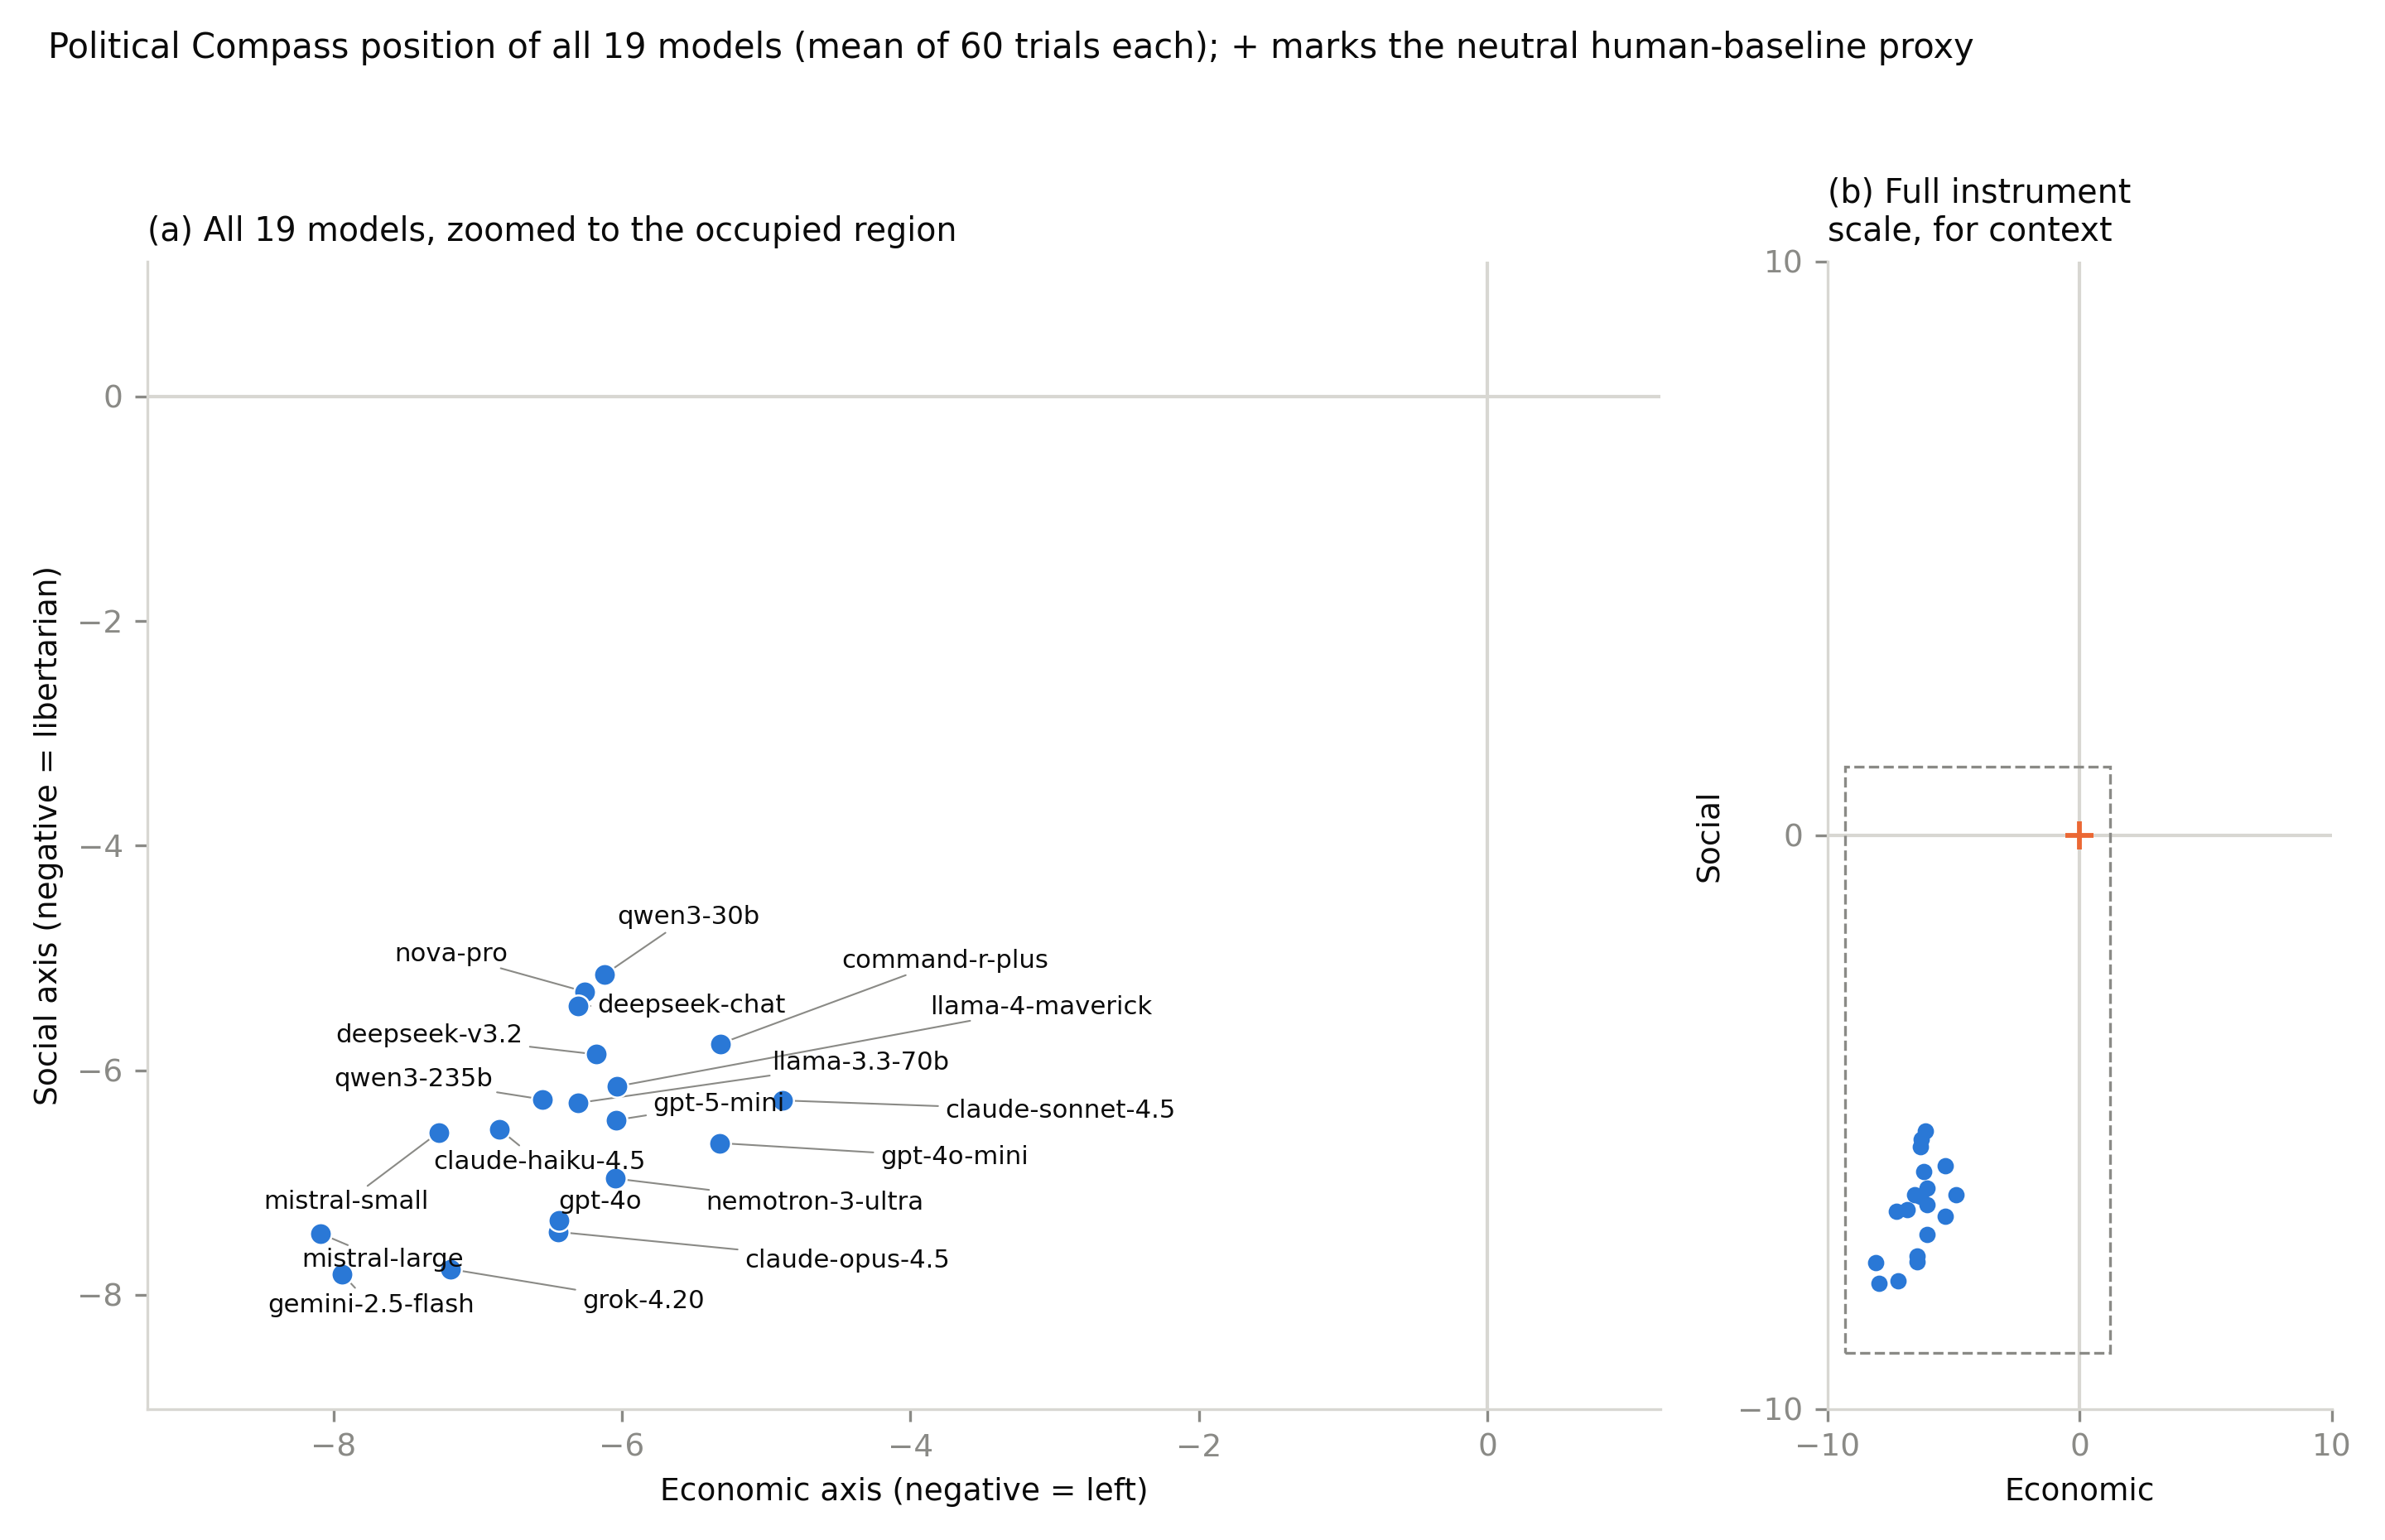
\includegraphics[width=0.95\textwidth]{figures/fig3_compass_scatter.png}
\caption{Political Compass position of all 19 models (mean of 60 trials each),
zoomed to the occupied region (a) with the full $-10$ to $10$ instrument
scale shown for context (b). The $+$ marks the neutral human-baseline proxy
used in Section~\ref{si:human-baseline}.}
\label{sfig:compass-scatter}
\end{figure}

\begin{figure}[H]
\centering
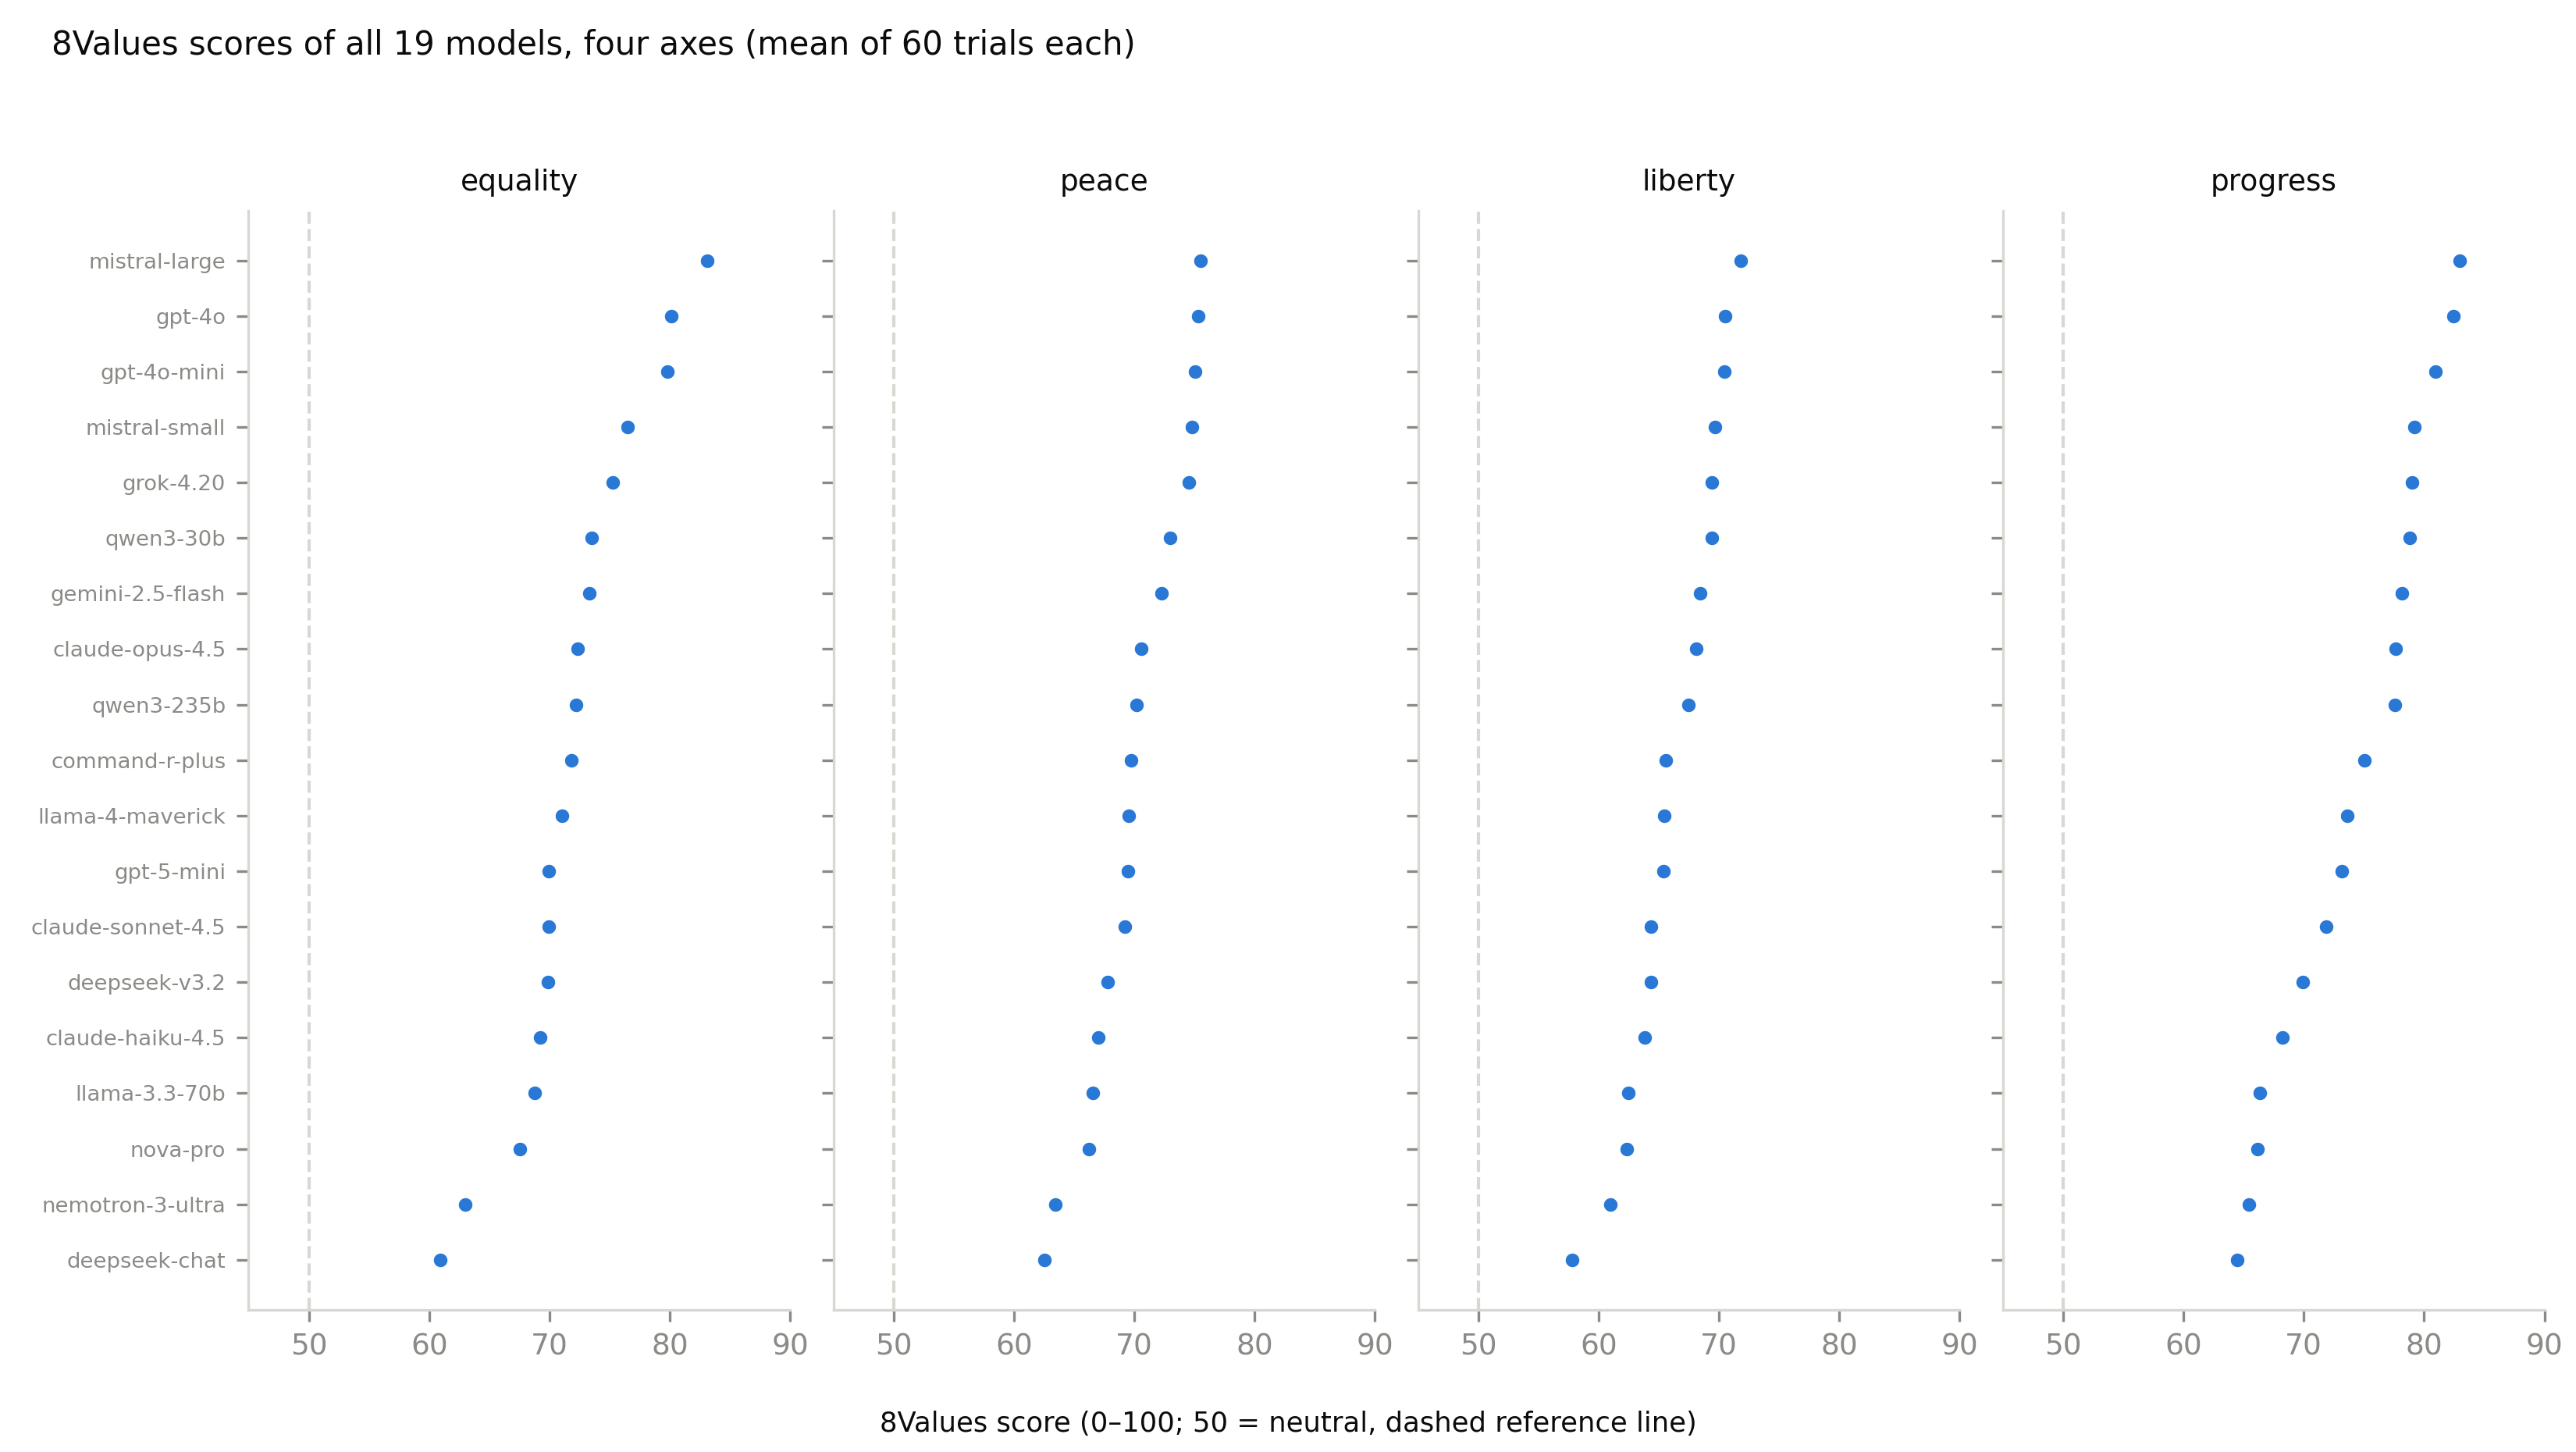
\includegraphics[width=\textwidth]{figures/fig4_8values_dotplot.png}
\caption{8Values scores of all 19 models on all four axes (mean of 60 trials
each), sorted independently within each panel; the dashed line marks the
instrument's neutral center-point (50).}
\label{sfig:8values-dotplot}
\end{figure}

\section{Omnibus Tests: Large, Robust Effects on Every Axis}

Table~\ref{stab:omnibus} reports the classical one-way ANOVA, Welch's ANOVA, and the
Kruskal-Wallis test, together with the omnibus eta-squared effect size, for each of
the six scored axes. All three tests agree at $p < .0001$ on every axis, and every
effect size is large ($\eta^2$ between $0.5625$ and $0.7263$). Shapiro-Wilk rejects
normality for a majority of the 19 groups on most axes (11 to 17 of 19 groups
non-normal, depending on axis), and Levene's test rejects equal variance on every
axis ($p<.0001$ throughout), which is why Welch's ANOVA and Kruskal-Wallis, not the
classical ANOVA, are treated as the primary evidence for these omnibus effects.

\begin{table}[H]
\centering
\caption{Omnibus tests across all 19 models, by axis. All three tests agree at every axis.}
\label{stab:omnibus}
\footnotesize
\begin{tabular}{llrrrr}
\toprule
Test & Axis & Classical $F$ & Welch $F$ & Kruskal-Wallis $H$ & $\eta^2$ \\
\midrule
8Values & Equality & 138.3 & 534.8  & 792.0 & 0.6896 \\
8Values & Peace    & 80.1  & 421.5  & 759.4 & 0.5625 \\
8Values & Liberty  & 89.3  & 459.2  & 753.5 & 0.5891 \\
8Values & Progress & 165.3 & 618.5  & 886.8 & 0.7263 \\
Pol.\ Compass & Economic & 124.8 & 2240.3 & 762.0 & 0.6670 \\
Pol.\ Compass & Social   & 163.3 & 1370.3 & 867.5 & 0.7239 \\
\bottomrule
\end{tabular}
\vspace{0.3em}

\footnotesize
\textit{Note:} all $p < .0001$ for all three tests, on every axis.
\end{table}

\section{Post-hoc Comparisons: Games-Howell as the Primary Test, Corrected for the Full Test Family}

With 19 groups, each axis has 171 pairwise comparisons, and six axes give a full
family of 1{,}026 pairwise tests reported across this paper. Because equal
variances are rejected on every axis, Games-Howell is treated as primary, with
Tukey HSD reported alongside. At raw $p<0.05$, Games-Howell finds between 121 and
144 of the 171 pairs significant per axis (equality: 142; peace: 136; liberty: 131;
progress: 144; economic: 121; social: 138), 812 of the 1{,}026 pairwise tests in
total. Applying a Benjamini-Hochberg false discovery rate correction across the
full family of 1{,}026 tests, rather than within each axis separately, leaves 809
of the 812 significant, a negligible change (equality: 142/142; peace: 136/136;
liberty: 131/131; progress: 142/144; economic: 120/121; social: 138/138): the
between-model differences reported here are not an artifact of running many
uncorrected tests. The two post-hoc tests mostly agree with each other as well:
wherever Tukey finds a different result than raw-$p$ Games-Howell, only 5 to 9
pairs per axis are significant under Tukey but not under Games-Howell, an artifact
of Tukey's equal-variance assumption rather than a real disagreement about the
larger pattern.

Several pairwise Games-Howell effect sizes (Hedges' $g$) on this dataset are very
large in magnitude, considerably larger than is typical for behavioral data. This
is not evidence of unusually large real differences so much as a consequence of
some models, particularly several Claude variants, having extremely low
within-model variance on some axes (Section~\ref{si:consistency}): dividing a
modest mean difference by a very small pooled standard deviation produces a large
standardized effect size even when the raw difference, on each instrument's own
$-10$-to-$10$ or 0-to-100 scale, is unremarkable. Readers should interpret the
reported Hedges' $g$ values alongside the raw mean differences in
Table~\ref{stab:descriptive}, not in isolation.

\section{Consistency: Range-Normalized Stability Varies by Model, not by Provider}
\label{si:consistency}

Ranking every model-axis combination by ISS (the Statistical Analysis subsection of the main-text Methods) shows that
the most and least consistent entries in the dataset are not concentrated in any
one provider, country, or size tier. Table~\ref{stab:iss-extremes} lists the ten
most and ten least consistent combinations out of all 114 (19 models $\times$ 6
axes).

\begin{table}[H]
\centering
\caption{Ten most and ten least consistent model-axis combinations by Ideological Stability Score (ISS). Lower ISS = more consistent.}
\label{stab:iss-extremes}
\footnotesize
\begin{tabular}{lr}
\toprule
Model (test/axis) & ISS \\
\midrule
\multicolumn{2}{l}{\textit{Most consistent}} \\
anthropic/claude-opus-4.5 (Pol.\ Compass/social) & 0.00 \\
anthropic/claude-opus-4.5 (8Values/peace)        & 7.62 \\
anthropic/claude-opus-4.5 (8Values/equality)     & 7.87 \\
anthropic/claude-sonnet-4.5 (Pol.\ Compass/social) & 8.26 \\
meta-llama/llama-3.3-70b (8Values/equality)      & 8.33 \\
anthropic/claude-sonnet-4.5 (Pol.\ Compass/economic) & 9.04 \\
amazon/nova-pro-v1 (Pol.\ Compass/economic)      & 9.21 \\
x-ai/grok-4.20 (8Values/peace)                    & 10.20 \\
meta-llama/llama-3.3-70b (8Values/peace)          & 12.11 \\
meta-llama/llama-3.3-70b (8Values/progress)       & 12.92 \\
\addlinespace
\multicolumn{2}{l}{\textit{Least consistent}} \\
qwen/qwen3-235b (8Values/equality)               & 34.14 \\
nvidia/nemotron-3-ultra (8Values/liberty)         & 35.58 \\
meta-llama/llama-4-maverick (8Values/liberty)     & 36.19 \\
deepseek/deepseek-chat (8Values/equality)         & 37.45 \\
google/gemini-2.5-flash (8Values/peace)           & 37.71 \\
nvidia/nemotron-3-ultra (8Values/peace)           & 40.50 \\
nvidia/nemotron-3-ultra (8Values/progress)        & 41.39 \\
nvidia/nemotron-3-ultra (8Values/equality)        & 42.76 \\
anthropic/claude-haiku-4.5 (Pol.\ Compass/economic) & 44.42 \\
anthropic/claude-opus-4.5 (Pol.\ Compass/economic) & 65.22 \\
\bottomrule
\end{tabular}
\end{table}

Table~\ref{stab:iss-extremes} shows only the twenty most extreme entries;
Figure~\ref{sfig:iss-distribution} shows the full distribution of all 114
ISS values, grouped by axis, and makes visible both the general spread
within each axis and the single high-leverage outlier
(anthropic/claude-opus-4.5's Political Compass economic score) discussed
below.

\begin{figure}[H]
\centering
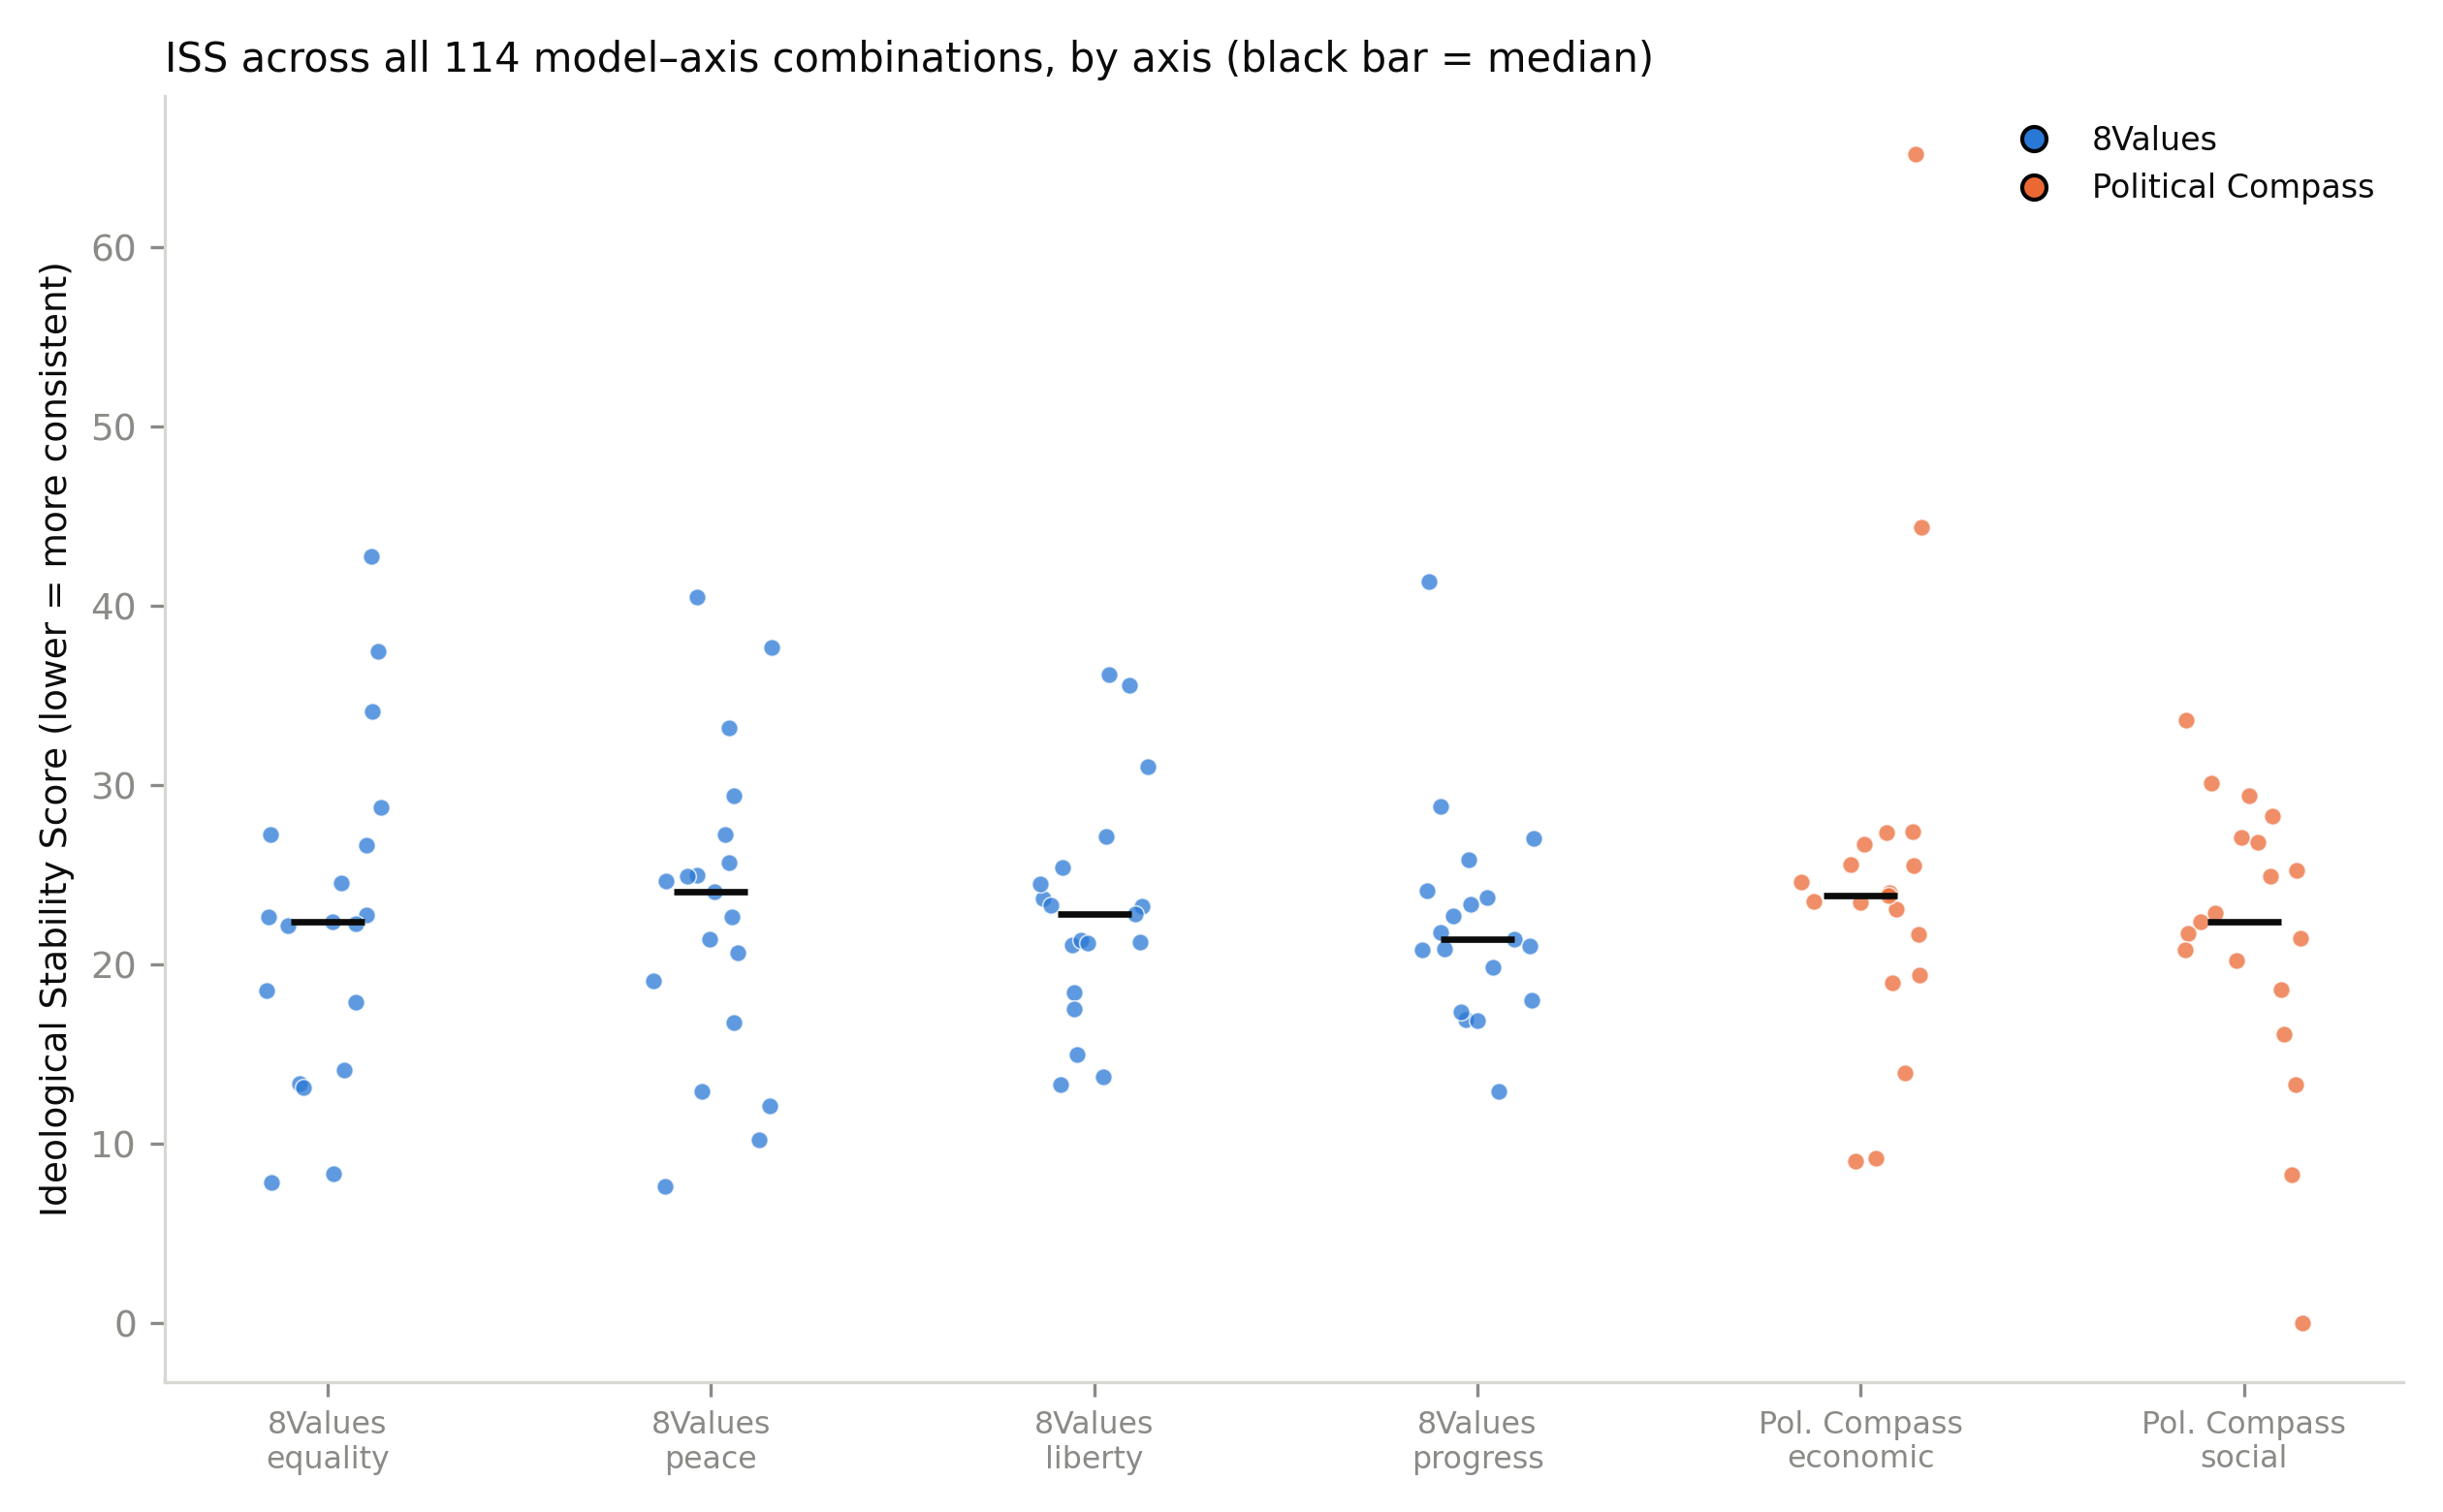
\includegraphics[width=0.85\textwidth]{figures/fig5_iss_distribution.png}
\caption{Ideological Stability Score for all 114 model--axis combinations,
grouped by axis. Each point is one model; the black bar marks the axis
median.}
\label{sfig:iss-distribution}
\end{figure}

anthropic/claude-opus-4.5 and meta-llama/llama-3.3-70b-instruct each appear three
times among the ten most consistent combinations, more than any other model, while
nvidia/nemotron-3-ultra-550b-a55b appears four times among the ten least
consistent. No provider is exclusively at either extreme: Claude variants appear
among both the single most consistent entry and, on a different axis, the single
least consistent entry in the entire dataset.

That last case illustrates the ISS range-normalization caveat from
the Statistical Analysis subsection of the main-text Methods directly. The Political Compass economic score of
anthropic/claude-opus-4.5 across its 60 trials took only two distinct values,
$-6.50$ and $-6.38$, an absolute range of $0.12$ on a $-10$-to-$10$ scale;
normalizing by that tiny self-range produces the highest ISS in the dataset
($65.22$) despite the underlying answers being, in absolute terms, essentially
constant. By contrast, the
same model's Political Compass social score was literally identical across all 60
trials ($-7.44$ every time, ISS $= 0.00$). Both figures describe a model giving
highly stable absolute answers; the ISS score for the economic axis should be read
as an artifact of the metric's normalization, not as evidence of erratic behavior.
anthropic/claude-haiku-4.5's economic-axis ISS ($44.42$) reflects a genuinely larger
absolute range ($-7.38$ to $-6.38$) and is a more straightforward instance of
comparatively lower consistency.

\section{Comparison Against a Human-Population Reference Point}
\label{si:human-baseline}

Beyond comparing models to each other, every one of the 114 model-axis
combinations (19 models $\times$ 6 axes) differs significantly from that
instrument's own neutral center-point (one-sample $t$-test against 0 for the two
Political Compass axes and against 50 for the four 8Values axes), and this holds
for all 114 tests even after a Benjamini-Hochberg false discovery rate correction.
Given that Gallup's 2024 Values and Beliefs poll finds the US public close to an
even three-way split between conservative, moderate, and liberal self-identification
on social issues, and only moderately right-of-center on economic issues
\cite{gallup2024values}, a neutral center-point is a reasonable, if bounded, proxy
for a human population reference (the Statistical Analysis subsection of the main-text Methods). Every model in this
study, without exception, differs significantly from that proxy, in the same
direction identified in the between-model comparisons above: left of center
economically and libertarian of center socially.

Statistical significance alone is a weak claim at $n=60$ trials per test, since
even a small, practically unremarkable deviation from center would clear
$p<0.05$ at that sample size. The effect sizes rule this out: computing a
one-sample Cohen's $d$ for each of the 114 tests (the standardized deviation of
a model's mean from the instrument's center-point) finds every finite value at
$|d|\geq 1.47$, comfortably past Cohen's conventional threshold for a
``large'' effect ($|d|\geq 0.8$) \cite{cohen1988}, with a median $|d|$ of
$11.92$ and a maximum of $106.74$ (one model-axis combination is excluded
from these summary statistics for having an effectively zero within-model
standard deviation, discussed in Section~\ref{si:consistency}). The deviation
from the neutral center-point is therefore not merely statistically
detectable but, on average, an order of magnitude larger than the
conventional threshold for a large effect.

\section{Prompt-Robustness Check: Magnitude Shifts, Direction Does Not}
\label{si:prompt-robustness}

Across the five-model, four-variant check (the Prompt-Robustness and Open-Ended-Generation Checks subsection of the main-text Methods),
prompt wording produced a statistically significant shift in 29 of 30
model-axis combinations tested (one-way ANOVA across the five prompt conditions,
$p<0.05$), and the effect size was large ($\eta^2 \geq 0.14$) in 28 of those 30,
with $\eta^2$ ranging from 0.02 to 0.75 (median 0.37). This is a genuine,
non-trivial finding, not a null result: instructional-wrapper wording measurably
moves scores for most models on most axes, consistent with Röttger et al.'s
critique that forced-choice political-typology evaluations are sensitive to
exactly how the task is framed \cite{rottger2024}.

What did not move is direction. Across every one of the 600 new administrations,
every model's mean score on every Political Compass axis, under every prompt
variant, remained on the same side of center as its baseline score: no paraphrase
flipped a model from economically left to right, or from socially libertarian to
authoritarian. The largest single shift observed was
\texttt{deepseek/deepseek-chat}'s 8Values equality score, ranging from 66.45 to
78.19 (an 11.7-point spread) across the five prompt conditions, still
comfortably on the equality (left) side of the 50-point center in every
condition. The
directional finding in Section 4.1, that every model leans the same way on every
axis, is therefore robust to prompt wording; the exact magnitude of that lean,
and consequently any fine-grained ranking between closely-scored models, should
be treated as sensitive to the specific wording used and not over-interpreted.

\section{Open-Ended-Generation Validation Arm}
\label{si:openended-results}

Across the 120 judged generations (the Prompt-Robustness and Open-Ended-Generation Checks subsection of the main-text Methods), the
correlation between a model's mean Political Compass score and its mean
judge-rated lean when writing open-endedly about matched-axis topics was weak
and not statistically significant on either axis (economic Pearson $r=-0.56$,
$p=0.32$; social $r=0.27$, $p=0.67$; $n=5$ models). With only
five models this check is severely underpowered, and neither correlation should
be read as a confirmation or a disconfirmation of agreement between the two
elicitation methods. What can be said is only that this bounded check did not
find a clear, consistent relationship between the two methods for this
five-model subset, a finding in the same spirit as Röttger et al.'s broader
point that forced-choice and open-ended elicitation can diverge
\cite{rottger2024}, and one that argues for a larger-scale version of this arm
(more models, more topics) before drawing a firm conclusion either way.

% =============================================================================


\section{Item-Response-Theory Reanalysis}
\label{si:irt}

The published Political Compass and 8Values scoring keys treat every item as
equally informative and cannot separate a model declining to engage from a
model holding a genuinely moderate position \cite{wachter2025irt}. We refit a
graded-response IRT model separately on each of the six axes (the four
8Values axes and the two Political Compass axes), using every item-level
response in the baseline dataset (19 models $\times$ 60 trials), and compare
the resulting latent trait ($\theta$) against each model's published axis
score.

\textbf{The published scores track the IRT-derived positions closely on five
of the six axes.} Spearman correlations between $\theta$ and the published
score range from $\rho=0.86$ to $\rho=0.94$ ($p<10^{-5}$ in every case) on
8Values equality, peace, liberty, and progress and on the Political Compass
social axis, with narrow Bland-Altman limits of agreement
(Table~\ref{stab:irt-summary}). \textbf{The exception is the Political
Compass economic axis}, where $\rho=0.64$ and the limits of agreement are
roughly twice as wide as on any other axis. That axis has only 11 items, the
fewest of the six, and half its information comes from just 2 of them
(Table~\ref{stab:irt-summary}) -- the published economic score for this
instrument rests on the fewest and least-distributed items in the study,
which is a specific, checkable reason to weight it less heavily than the
other five axes rather than a general indictment of the scoring approach.

\textbf{Information is concentrated in a minority of items on every axis.}
Between 4 and 12 items (out of 11 to 50 per axis) carry half of each axis's
total discrimination, and the top decile of items by discrimination carries
24-33\% of it. A small, identifiable subset of items is doing most of the
work of separating models on every axis we fit, on both instruments.

\textbf{Neutral-response rates vary roughly five-fold across models on
8Values} (9\% to 52\% of items answered at the scale midpoint), which is the
avoidance behaviour Wachter et al. (2025) predicts: at least part of the
apparent centrism in the most avoidant models is a refusal to commit to
either pole rather than a moderate position, and it is not evenly distributed
across the cohort. We do not have a validated way to convert a neutral-rate
estimate into a bias correction for the published score, so we report it as a
per-model caveat rather than an adjustment.

\begin{table}[H]
\centering
\caption{IRT reanalysis summary by axis. $\rho$ is the Spearman correlation
between the IRT latent trait and the published axis score across the 19
models; LoA is the Bland-Altman 95\% limits of agreement, in the published
score's own units after within-axis standardization; ``items for half
info.'' is the minimum number of items whose summed discrimination reaches
half the axis total.}
\label{stab:irt-summary}
\footnotesize
\begin{tabular}{llrrrr}
\toprule
Instrument & Axis & Items & $\rho$ & LoA & Items for half info. \\
\midrule
8Values & Equality & 22 & 0.91 & $\pm 0.83$ & 4 \\
8Values & Peace & 24 & 0.86 & $\pm 0.88$ & 6 \\
8Values & Liberty & 37 & 0.92 & $\pm 0.61$ & 7 \\
8Values & Progress & 33 & 0.88 & $\pm 0.81$ & 7 \\
Political Compass & Economic & 11 & 0.64 & $\pm 1.27$ & 2 \\
Political Compass & Social & 50 & 0.94 & $\pm 0.63$ & 12 \\
\bottomrule
\end{tabular}
\end{table}

\section{Multi-trait multi-method matrix}

The full correlation matrix behind the convergent-validity result in the main
text is shown in main-text Fig.~3 and Table~2. Convergent coefficients (same
construct, different instrument) average $r=-0.26$; discriminant coefficients
(different construct, same instrument) average $r=+0.52$. The four 8Values axes
correlate with one another at mean $r=0.71$, consistent with a single dominant
general factor rather than four separable traits.



\section{Display items moved from the main text}

\begin{figure}[H]
  \centering
  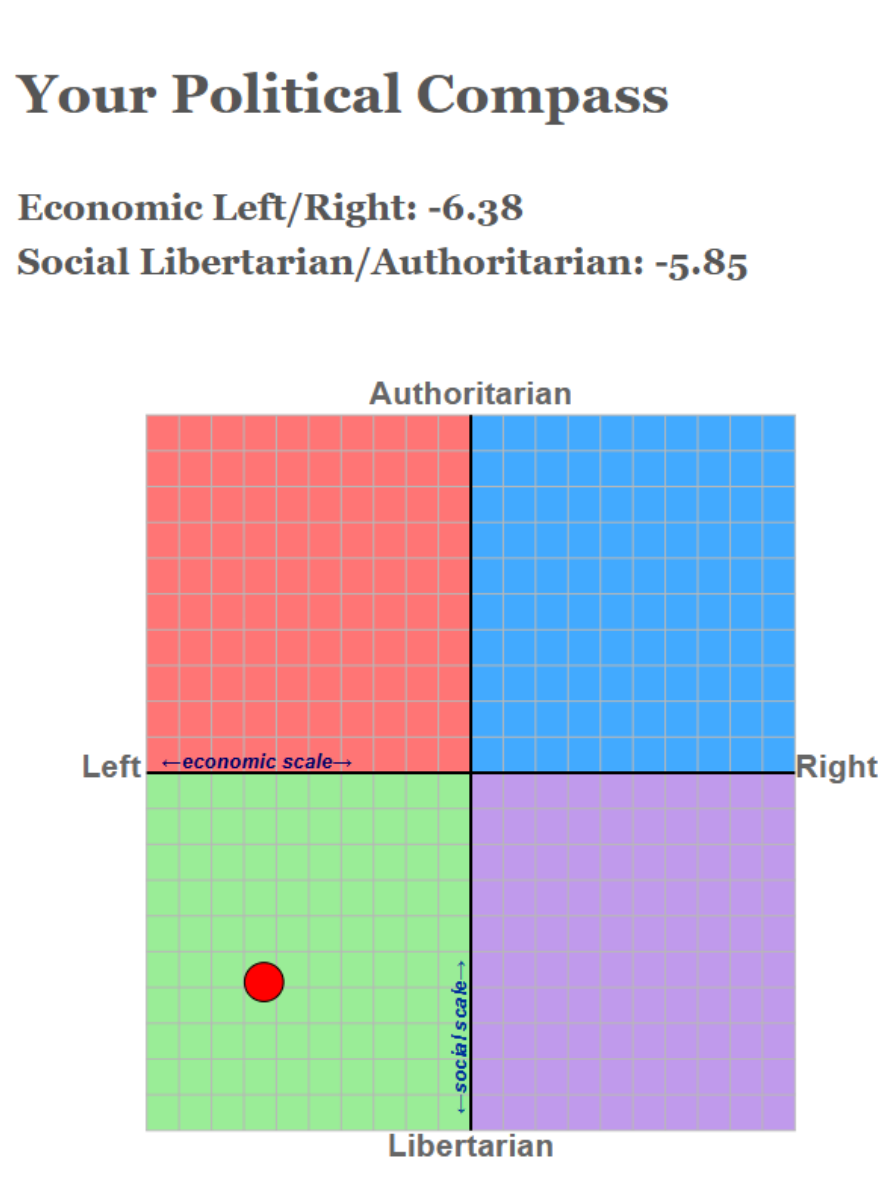
\includegraphics[width=0.55\textwidth]{figures/fig1_political_compass.png}
  \caption{Example Political Compass output for a single trial.}
  \label{sfig:polcompass}
\end{figure}
\begin{figure}[H]
  \centering
  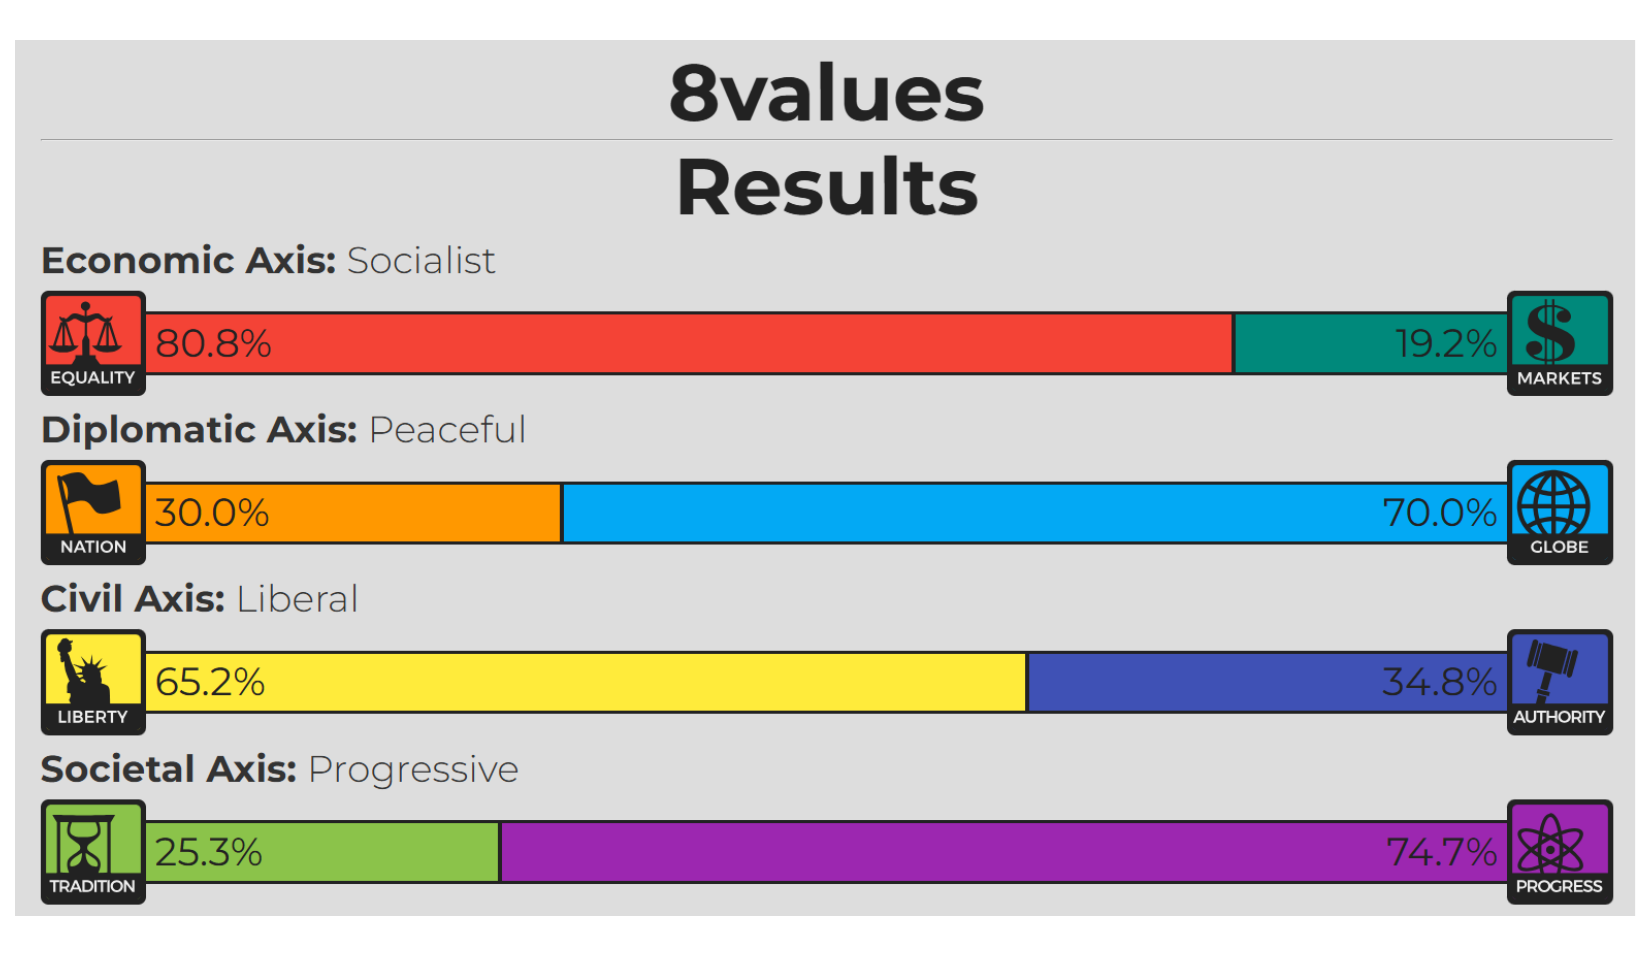
\includegraphics[width=0.85\textwidth]{figures/fig2_8values.png}
  \caption{Example 8Values output for a single trial.}
  \label{sfig:8values}
\end{figure}
\begin{table}[H]
\centering
\caption{Collection completion rate and cost by model (both tests combined, 120 administrations/model).}
\label{stab:collection-summary}
\footnotesize
\begin{tabular}{lrr}
\toprule
Model & Completion rate & Cost \\
\midrule
amazon/nova-pro-v1 & 100\% & \$0.31 \\
anthropic/claude-haiku-4.5 & 100\% & \$0.42 \\
anthropic/claude-opus-4.5 & 100\% & \$1.95 \\
anthropic/claude-sonnet-4.5 & 100\% & \$1.42 \\
cohere/command-r-plus-08-2024 & 100\% & \$0.98 \\
deepseek/deepseek-chat & 100\% & \$0.09 \\
deepseek/deepseek-v3.2 & 100\% & \$0.02 \\
google/gemini-2.5-flash & 100\% & \$0.21 \\
meta-llama/llama-3.3-70b-instruct & 100\% & \$0.04 \\
meta-llama/llama-4-maverick & 100\% & \$0.07 \\
mistralai/mistral-large-2512 & 100\% & \$0.11 \\
mistralai/mistral-small-3.2-24b-instruct & 100\% & \$0.02 \\
nvidia/nemotron-3-ultra-550b-a55b & 100\% & \$1.38 \\
openai/gpt-4o & 100\% & \$0.84 \\
openai/gpt-4o-mini & 100\% & \$0.04 \\
openai/gpt-5-mini & 100\% & \$0.59 \\
qwen/qwen3-235b-a22b & 100\% & \$0.49 \\
qwen/qwen3-30b-a3b & 100\% & \$0.14 \\
x-ai/grok-4.20 & 100\% & \$0.18 \\
\midrule
Total & 100\% (2{,}280/2{,}280) & \$9.30 \\
\bottomrule
\end{tabular}
\end{table}
\begin{table}[H]
\centering
\caption{Multi-trait multi-method coefficients across the 19 models. Convergent validity requires that the same construct measured by two instruments correlate more strongly than two different constructs measured by the same instrument. It does not.}
\label{stab:mtmm}
\begin{tabular}{llr}
\toprule
Type & Pair & $r$ \\
\midrule
Convergent & 8values:economic vs political\_compass:economic & -0.005 \\
Convergent & 8values:social vs political\_compass:social & -0.506 \\
Discriminant & 8values:economic vs 8values:social & +0.490 \\
Discriminant & political\_compass:economic vs political\_compass:social & +0.549 \\
\midrule
\textbf{Mean convergent} & & \textbf{-0.255} \\
\textbf{Mean discriminant} & & \textbf{+0.520} \\
\bottomrule
\end{tabular}
\end{table}

\bibliographystyle{unsrt}
\bibliography{references}
\end{document}
